
\section{Block-Diagram Algebra}

%%%%%%%%%%%%%%% Block Diagram Syntax %%%%%%%%%%%%%%%%%%%%%%%%%%
\begin{frame}[fragile]{Block-Diagram Algebra}
Programming by patching is familiar to musicians :

\begin{figure}[h]
\centering
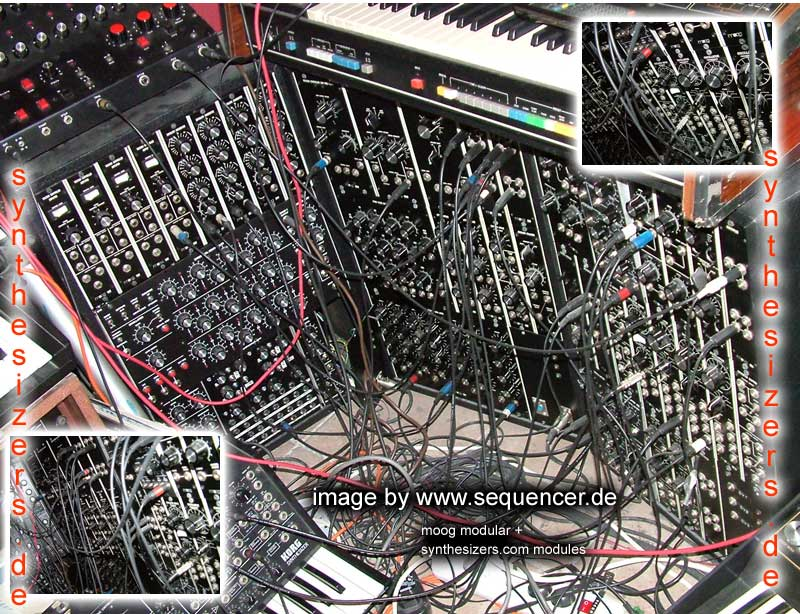
\includegraphics[height=4cm]{images/moog}
\hspace{0.1cm}
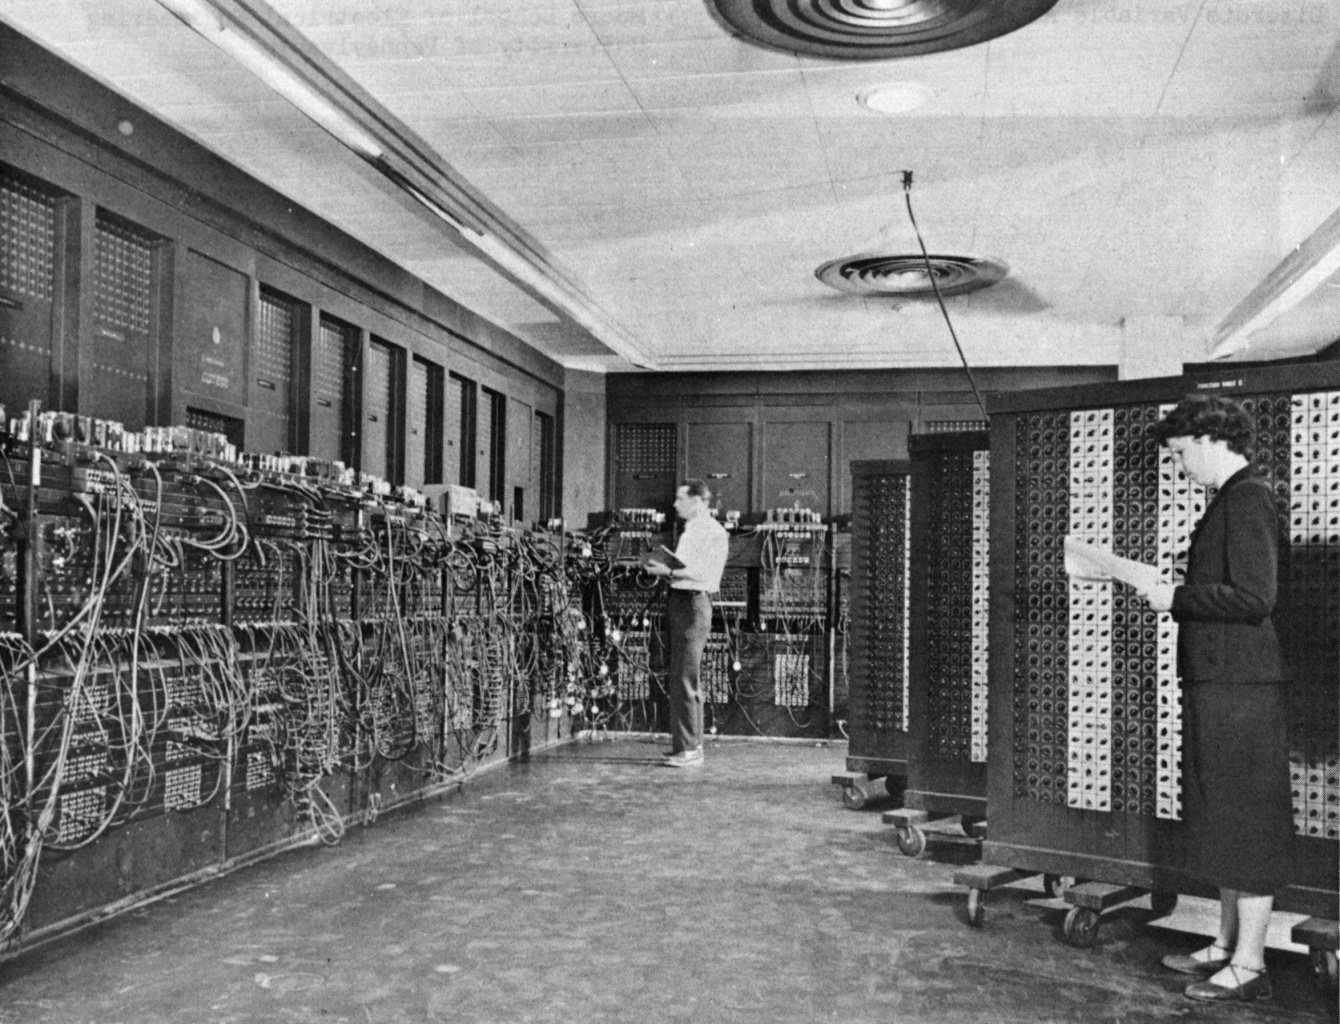
\includegraphics[height=4cm]{images/eniac}
\label{figure:moog}
\end{figure}

\end{frame}


% %%%%%%%%%%%%%%% Block Diagram Syntax %%%%%%%%%%%%%%%%%%%%%%%%%%
% \begin{frame}[fragile]{Block-Diagram Algebra}
% Programming by patching was also used to program the first electronic computers :
% 
% \begin{figure}[h]
% \centering
% 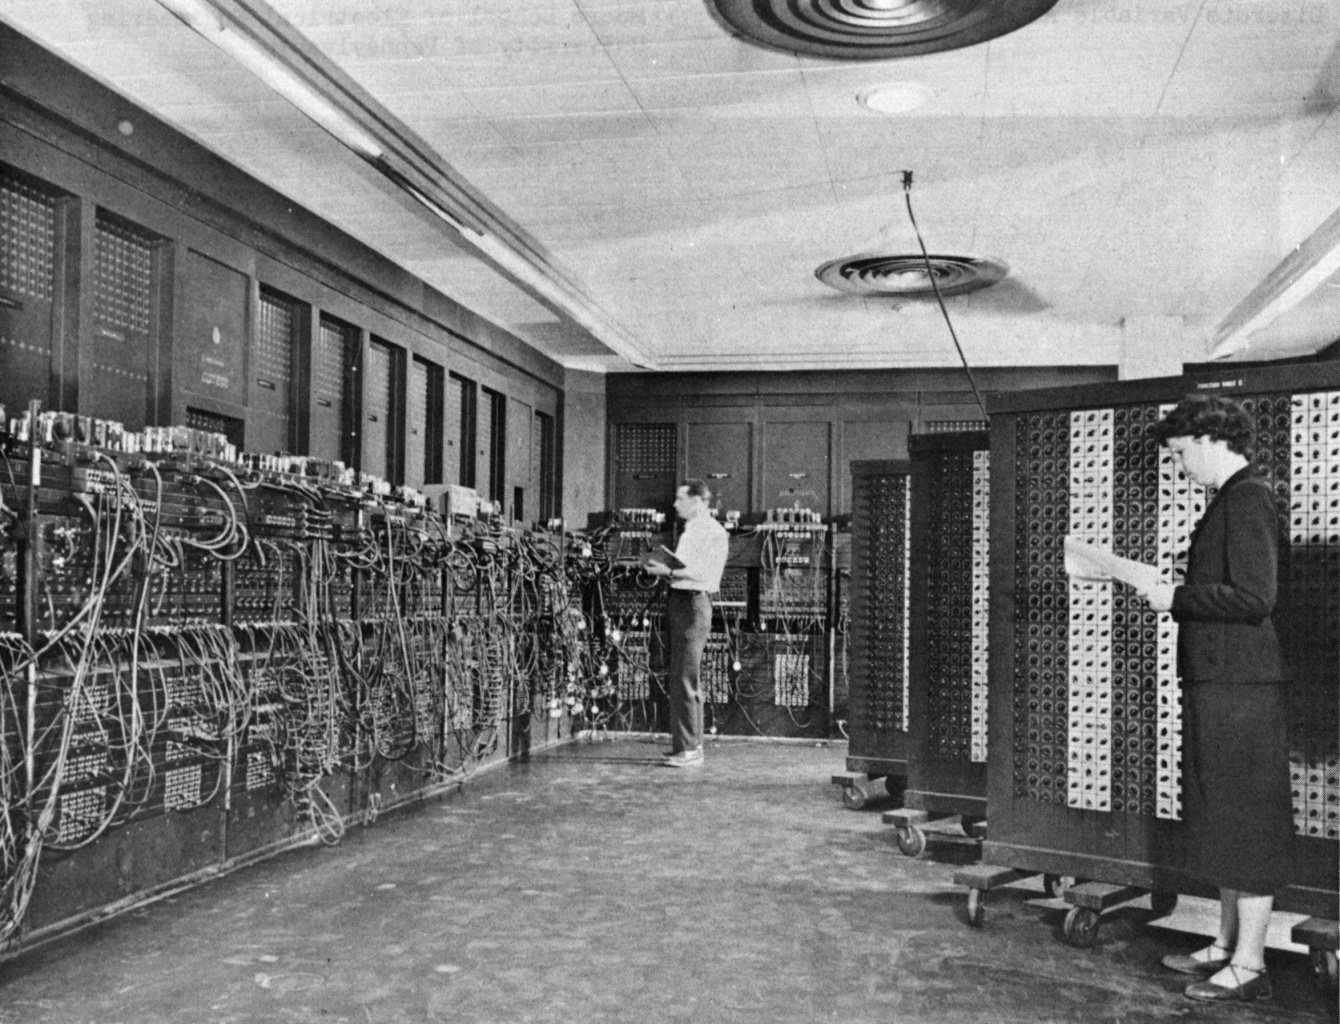
\includegraphics[height=5cm]{images/eniac}
% \caption{the ENIAC computer}
% \label{figure:eniac}
% \end{figure}
% \end{frame}
% 

%%%%%%%%%%%%%%% Block Diagram Syntax %%%%%%%%%%%%%%%%%%%%%%%%%%
\begin{frame}[fragile]{Block-Diagram Algebra}
Today programming by patching is widely used in Visual Programming Languages like Max/MSP:

\begin{figure}[h]
\centering
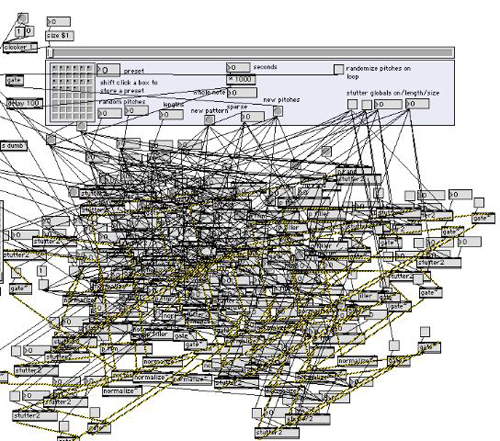
\includegraphics[height=6cm]{images/patch-max-complex}
\caption{Block-diagrams can be a mess}
\label{figure:mess}
\end{figure}
\end{frame}


%%%%%%%%%%%%%%% Block Diagram Syntax %%%%%%%%%%%%%%%%%%%%%%%%%%
\begin{frame}[fragile]{Block-Diagram Algebra}
Faust allows structured block-diagrams

\begin{figure}[h]
\centering
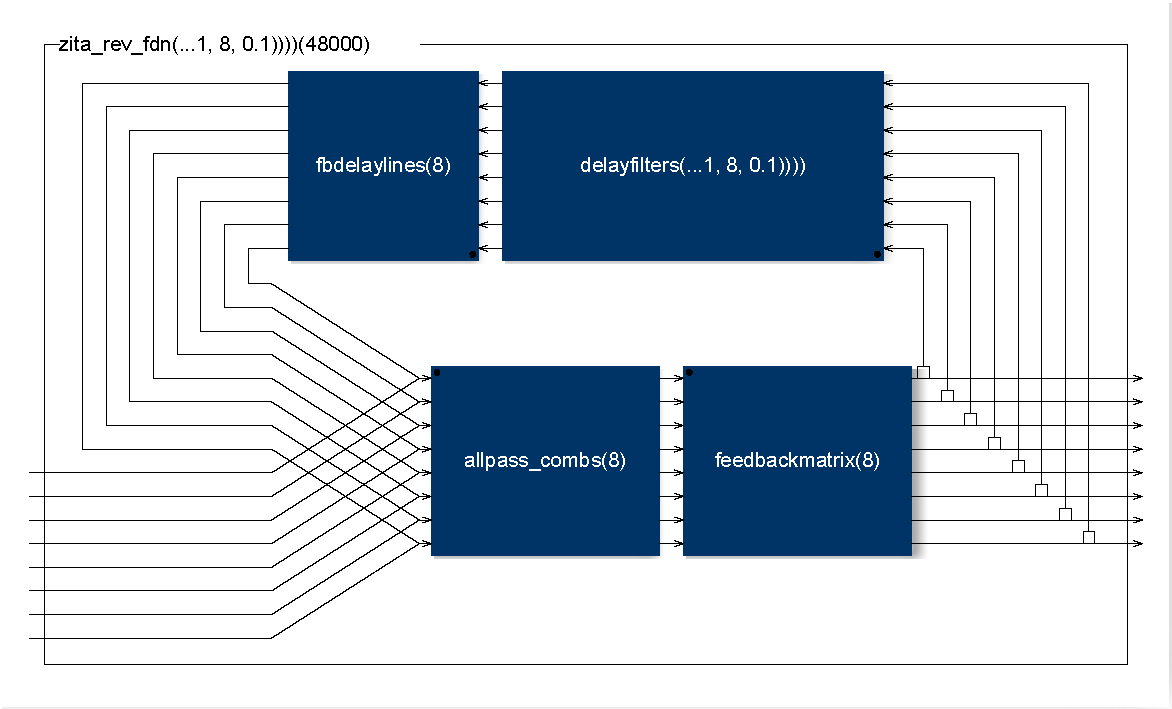
\includegraphics[height=6cm]{images/zita-diagram}
\caption{A complex but structured block-diagram}
\label{figure:matrix}
\end{figure}
\end{frame}


%%%%%%%%%%%%%%% Block Diagram Syntax %%%%%%%%%%%%%%%%%%%%%%%%%%
\begin{frame}[fragile]{Block-Diagram Algebra}
\framesubtitle{Faust syntax is based on a \emph{block diagram algebra}} 

	\begin{exampleblock}{5 Composition Operators}
		\begin{itemize}
		\item \lstinline'(A~B) ' recursive composition (priority 4)
		\item \lstinline'(A,B) ' parallel composition (priority 3)
		\item \lstinline'(A:B) ' sequential composition (priority 2)
		\item \lstinline'(A<:B)' split composition (priority 1)
		\item \lstinline'(A:>B)' merge composition (priority 1)
		\end{itemize}
	\end{exampleblock}
	
	\begin{exampleblock}{2 Constants}
		\begin{itemize}
		\item \lstinline'!' cut
		\item \lstinline'_' wire
		\end{itemize}
	\end{exampleblock}


\end{frame}


%%%%%%%%%% parallel composition %%%%%%%%%%%%%%%%%%
\begin{frame}[fragile]{Block-Diagram Algebra}
\framesubtitle{Parallel Composition}
The \emph{parallel composition} $(A,B)$ is probably the simplest one. It places the two block-dia\-grams one on top of the other, without connections. 

\begin{figure}[h]
\centering
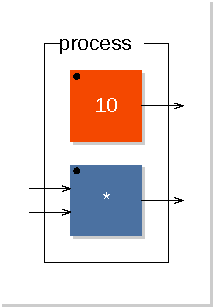
\includegraphics[scale=0.5]{images/par1}
\caption{Example of parallel composition  \lstinline'(10,*)'}
\label{figure:par1}
\end{figure}

\end{frame}

%%%%%%%%%% sequential composition %%%%%%%%%%%%%%%%%%
\begin{frame}[fragile]{Block-Diagram Algebra}
\framesubtitle{Sequential Composition}
The \emph{sequential composition} $(A:B)$ connects the outputs of  $A$ to the inputs of  $B$.  $A[0]$ is connected to $[0]B$,   $A[1]$ is connected to $[1]B$, and so on. 

\begin{figure}[h]
\centering 
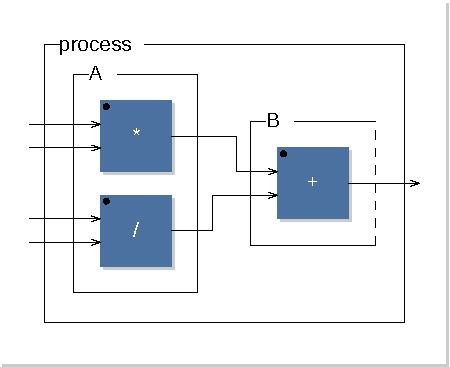
\includegraphics[scale=0.5]{images/seq1}
\caption{Example of sequential composition  \lstinline'((*,/):+)' } 
\label{figure:seq1}
\end{figure}

Note that the number of outputs of $A$ must be equal to the number of inputs of $B$.
\end{frame}


%%%%%%%%%% split composition %%%%%%%%%%%%%%%%%%
\begin{frame}[fragile]{Block-Diagram Algebra}
\framesubtitle{Split Composition}
The \emph{split composition} $(A<:B)$ operator is used to distribute $A$ outputs
to $B$ inputs.

\begin{figure}[h]
\centering 
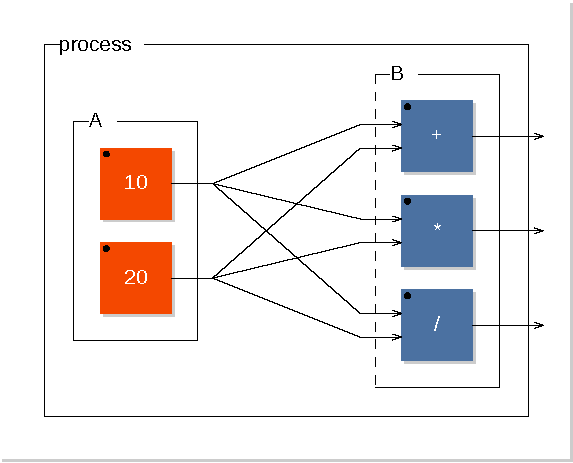
\includegraphics[scale=0.5]{images/split1} 
\caption{example of split composition   \lstinline'((10,20) <: (+,*,/))'}  
\label{figure:split1}
\end{figure}

\end{frame}


%%%%%%%%%% merge composition %%%%%%%%%%%%%%%%%%
\begin{frame}[fragile]{Block-Diagram Algebra}
\framesubtitle{Merge Composition}
The \emph{merge composition} $(A:>B)$ is used to connect several outputs
of  $A$ to the same inputs of $B$. 

\begin{figure}[h]
\centering 
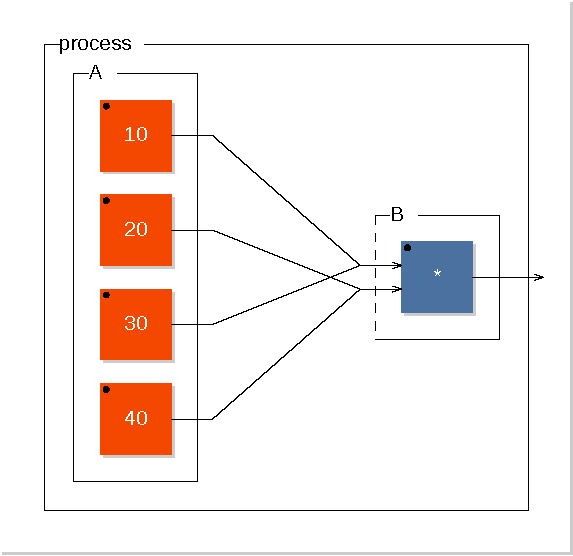
\includegraphics[scale=0.5]{images/merge1} 
\caption{example of merge composition \lstinline'((10,20,30,40) :> *)'}  
\label{figure:merge1}
\end{figure}
 
\end{frame}


%%%%%%%%%% recursive composition %%%%%%%%%%%%%%%%%%
\begin{frame}[fragile]{Block-Diagram Algebra}
\framesubtitle{Recursive Composition}
    The \emph{recursive composition} \lstinline'(A~B)' is used to create cycles in the block-diagram in order to express recursive computations.
    
    \begin{figure}[h]
    \centering 
    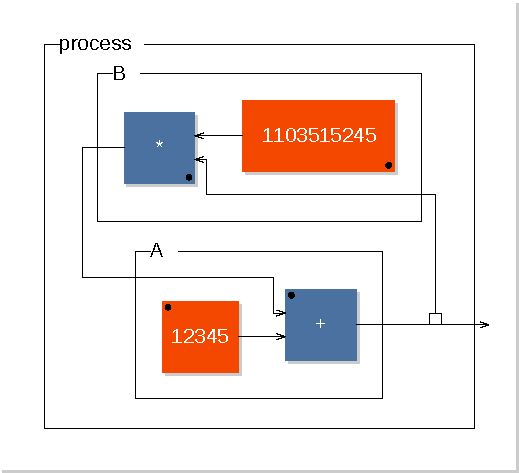
\includegraphics[scale=0.5]{images/rec1} 
    \caption{example of recursive composition \lstinline'+(12345) ~ *(1103515245)'}  
    \label{figure:rec1}
    \end{figure}
\end{frame}
 

%%%%%%%%%%% comparing synatx %%%%%%%%%%%%%%%%%%
%\begin{frame}[fragile]{Block-Diagram Syntax}
%\framesubtitle{Same expression in Lambda-Calculus, FP and Faust}

%\pause
%\begin{exampleblock}{Lambda-Calculus}
%\lstinline'\x.\y.(x+y,x*y) 2 3'
%\end{exampleblock}

%\pause
%\begin{exampleblock}{FP/FL (John Backus)}
%\lstinline'[+,*]:<2,3>'
%\end{exampleblock}

%\pause
%\begin{exampleblock}{Faust}
%\lstinline'2,3 <: +,*'
%\end{exampleblock}
%\end{frame}

